\documentclass{article}
\usepackage{pgf}
\usepackage{xcolor}
\usepackage{amsmath}
\usepackage{amssymb}  % put in preamble
\usepackage{tikz}
\usepackage{mathtools}
\usepackage{tkz-euclide}
\usepackage{amsfonts}
\usepackage{graphicx}
\graphicspath{{./assets/}}

\numberwithin{equation}{section}
\title{Gravity Demo}
\author{Martin N. Håvardsen}
\date{\today}

\begin{document}
\maketitle
\begin{center}
\includegraphics[width=0.8\textwidth]{ARTSTYLE.png}\\
\end{center}
\section{Generell protokoll}
\begin{enumerate}
  \item Finn alle retningsvektorer for gravitasjonskreftene.
  \item Regn ut $\vec a$ 
\end{enumerate}
\includegraphics[width=1\textwidth]{update_acceleration_CODE.png}
\begin{figure}[h]
\centering
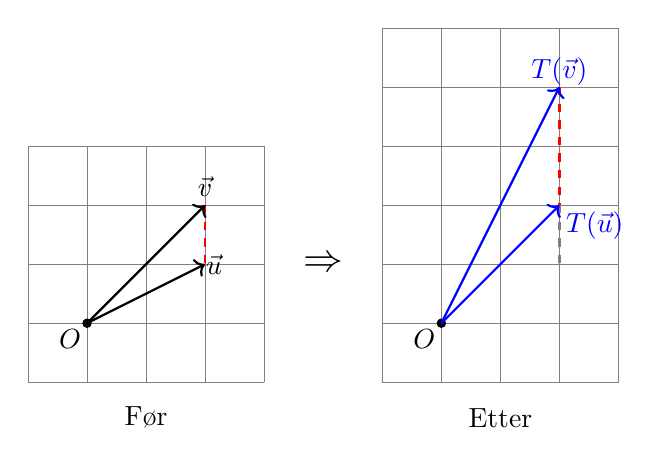
\begin{tikzpicture}[scale=1.5, every node/.style={inner sep=0pt}]
  % Left picture
  \begin{scope}[shift={(0,0)}]
    \draw[step=0.5cm,gray,very thin] (-0.5,-0.5) grid (1.5,1.5);
    \draw[dashed, thick, red] (1,1) -- (1,0.5);
    \filldraw[black] (0,0) circle (1pt) node [below left=0.1] {$O$};
    \draw[thick,->] (0,0) -- (1,1) node[above=0.1cm] {$\vec{v}$};
    \draw[thick,->] (0,0) -- (1,0.5) node[right] {$\vec{u}$};
    \node at (0.5,-0.8) {Før};
  \end{scope}

  % Arrow in the middle
  \node at (2,0.5) {\Large $\Rightarrow$};

  % Right picture
  \begin{scope}[shift={(3,0)}]
    \draw[step=0.5cm,gray,very thin] (-0.5,-0.5) grid (1.5,2.5);
    \draw[dashed, thick, red] (1,2) -- (1,1);
    \draw[dashed, thick, gray] (1,1) -- (1,0.5);
    \filldraw[black] (0,0) circle (1pt) node [below left=0.1cm] {$O$};
    \draw[thick,->,blue] (0,0) -- (1,2) node[above] {$T(\vec{v})$};
    \draw[thick,->,blue] (0,0) -- (1,1) node[below right=0.1cm] {$T(\vec{u})$};
    \node at (0.5,-0.8) {Etter};
  \end{scope}
\end{tikzpicture}
  \caption{Transformeringen av $\vec v$ og $\vec u$ under $T$}
\end{figure}
% collision drawing
\begin{figure}[h]
  \centering
  \begin{tikzpicture}[scale=1]
    \begin{scope}[shift={(0,0)}]
      \begin{scope}[shift={(0,-0.4)}, rotate=30]
        \draw (0,0) circle (1) node[left]{$A$};
        \draw [thin, ->, blue] (-0.8,1.2) -- (0.8,1.2) node[midway, above=0.1]{$\vec v_{A0}$};
      \end{scope}
      \draw [thick, red] (2,2) -- (2,-1) node[above right=0.1]{$B$};
      \node[scale=1, circle] (B) at (0,-2){Før};
    \end{scope}
    %\node[scale=2, circle] (A) at (4,0){$\implies$};
    \begin{scope}[shift={(4.5,0)}]
      \begin{scope}[shift={(1,0.4)},rotate=30]
        \draw (0,0) circle (1) node[left]{$A$};
        %\draw [thin, ->, blue] (-1.2,-1.2) -- (0.4,-1.2) node[midway, below]{$\vec v_{A0}$};
      \end{scope}
      % Triangle points
      \coordinate (A1) at (0,0);
      \coordinate (B1) at (4,0);
      \coordinate (C1) at (2,3);
      \draw [thick, red] (2,2) -- (2,-1) node[above right=0.1]{$B$};
      \node[scale=1, circle] (B) at (0.8,-2){Under kontakt};
    \end{scope}
    \begin{scope}[shift={(9.5,0)}]
      \begin{scope}[shift={(0,1.2)}, rotate=-30, xscale=-1]
        \draw (0,0) circle (1) node[left]{$A$};
        \draw [thin, ->, blue] (-0.8,1.2) -- (0.8,1.2) node[midway, above]{$\vec v_A$};
      \end{scope}
      \draw [thick, red] (2,2) -- (2,-1) node[above right=0.1]{$B$};
      \node[scale=1, circle] (B) at (0.4,-2){Etter};
    \end{scope}
  \end{tikzpicture}
  \caption{Kollisjon mellom objekt $A$ og barriere $B$}
\end{figure}
\begin{figure}[h]
  \centering
  \begin{tikzpicture}[scale=1]
    \coordinate (A1) at (-5,2);
    \coordinate (A2) at (-5,-2);
    \coordinate (O) at (0,0);
    \coordinate (B1) at (5,2);
    \coordinate (B2) at (5,-2);
    \coordinate (E1) at (-5,0);
    \coordinate (E2) at (5,0);
    \draw[red, thick, ->] (O) -- (0,1) node[above, right]{$\vec n$};
    \draw[blue] (A1) -- (O);
    \draw[blue, thick, ->] (A1) -- ($(A1)!0.4!(O)$) node[above, right]{$\vec v_{A0}$};
    \draw[blue, dashed] (O) -- (B1);
    \draw[blue, dashed] (O) -- (B2);
    \draw (E1) -- (E2);
    \pic["$\alpha$", draw, angle radius=1.6cm] {angle = A1--O--E1};
    \pic["$\beta$", draw, angle radius=1.6cm, dashed] {angle = E2--O--B1};
  \end{tikzpicture}
  \caption{Speiling}
\end{figure}
\begin{table}[h]
  \centering
  \begin{tabular}{|l|l|l|}
  \hline
  \textbf{Funksjon} & \textbf{input} &\textbf{output} \\
  \hline
  \texttt{update\_objects} &  & \\
  \hline
    \texttt{add\_object\_with\_vel} &\texttt{pos} : \textit{vec2}&\\& \texttt{color} : \textit{vec3}&\\& \texttt{mass} : \textit{float}&\\& \texttt{vel} : \textit{vec2} & \\
  \hline
    \texttt{add\_object} &\texttt{pos} : \textit{vec2}&\\& \texttt{color} : \textit{vec3}&\\& \texttt{mass} : \textit{float}& \\
  \hline
  \texttt{transform\_window\_to\_plane} &\texttt{v} : \textit{vec2} & transformed v \\
  \hline
  \texttt{transform\_plane\_to\_window} &\texttt{v} : \textit{vec2} &transformed v \\
  \hline
    \texttt{transform\_plane\_to\_window\_tuplet} &\texttt{v} : \textit{vec2}  & transformed v\\
  \hline
    \texttt{draw\_circle\_in\_plane} &\texttt{window} : \textit{pygame.surface}&\\& \texttt{color} : \textit{vec3}&\\& \texttt{pos} : \textit{vec2}&\\& \texttt{rad} : \textit{uint}&\\& \texttt{outline\_thickness} : \textit{uint} & \\
  \hline
  \texttt{handle\_mb2} & & \\
  \hline
\end{tabular}
  \caption{Matrise med funksjoner}
\end{table}
\clearpage
\section{Feiltagelser under fysikk prøven og deres trekk}
\begin{description}
  \item [Enheter] Husk å skrive enheter under regning. Dette inkluderer delregninger.
  \item [Misforståing] Husk å lese spørsmålene med kirurgisk nøyaktighet.
  \item [Tidsdisponering] Husk å bruk tiden effektivt.
    Det ble gitt 30 minutt per oppgave. Ikke sjekk over det du har gjort for mye, det er bedre å få skrive mye ok enn lite, korrekt.
  \item [Symbolsk forståing] I formel derivasjonsoppgaven var det viktig å ikke bruke tid på å forstå uttrykkene, men heller å rent algebraisk løse for bestemte variabler.
    Ikke tenk for mye!
  \item [Mangel på klare mål] Husk å fastsette målet for å mest effektivt oppnå det.
  \item [Dårlig hukommelse] Alle formler må komme med en gang man trenger dem.
    Ikke bruk tid på å huske relevante formler, eller på å finne ut hva som kan være relevant.
  \item [Formelutleding] Dersom man får et uttrykk som er ulikt det ønskede uttrykket, så er det ikke nødvendigvis feil.
    Sjekk om det er noen uønskede variabler i uttrykket.
    Kanskje kan du substituere inn noe for å oppnå ønsket uttrykk.
\end{description}
\section{Formler}
\subsection{Formler i kapittel 1}
\textbf{Konstant fart}
\[v=at+v_0\]
\[s=\frac{v+v_0}{2}t\]
\[s=\frac 1 2 at^2+v_0t\]
\[v^2-v_0^2=2as\]
%\hrule
\textbf{Funksjoner}
\[a(t)=v'(t)=s''(t)\]
%\hrule
\textbf{Dekomponering}
\[F_x=F\cos\theta\]
\[F_y=F\sin\theta\]
%\hrule
\textbf{Newtons lover}
\[\Sigma \vec F = \vec 0 \iff \vec v = k, \text{$k$ er konstant og kan være lik 0}\]
\[\Sigma \vec F = m\vec a\]
\[\text{Når A virker på B med kraft $\vec F$, virker $\vec F^*$ på A}\hspace{1cm}\hfill\vec F^*=-\vec F\]
\textbf{Energi og arbeid}
\[W=\vec F\cdot\vec s=F\cdot s\cdot \cos\theta\hspace{1cm}\text{$\theta=$vinkel mellom $\vec F$ og $\vec s$}\]
\[W_{\Sigma F}=\Delta E_k\hspace{1cm} \text{$W_{\Sigma F}=$arbeidet fra $\Sigma F$}\]
\[W=\int_A^B F(s)ds\]
\textbf{Bevaring}
\[\text{berre tyngdekrafta gjør et arbeid}\implies E=E_0\implies E_p+E_k=E_{p0}+E_{k0}\]
\[E=E_0+W_A \hspace{1cm}\text{$W_A$ er andre krefter enn tyngdekrafta som gjør arbeid}\]
\[\Sigma F, \text{for et system}, = 0 \implies \vec\rho=\vec\rho_0\]
\textbf{Error}
\par
\small{\textbf{Merk!}
Høyere grannsemd i målingene gir en mer korrekt gjennomsnittsverdi. Høyere presisjon i målingene gir mindre spredelse i resultatene.}
\[x=\overline x\pm \Delta x\]
\[\overline x =\frac{\text{summen av målingene}}{\text{talet på målinger}}\]
\[\Delta x=\frac{x_{\text{maks}}-x_{\text{min}}}{2}\]
\[\text{Relative error}=\frac{\Delta x}{x}\]
\[s=x\pm y\implies \Delta s=\Delta x + \Delta y\]
\[\rho=x\cdot y^{\pm 1}\implies\frac{\Delta\rho}{\rho}=\frac{\Delta x}{x}+\frac{\Delta y}{y}\]
\subsection{Formler i kapittel 2}
\subsection{Formler i kapittel 3}
\section{Øving}
\subsection{Kapittel 2}
\begin{table}[h]
  \centering
  \begin{tabular}{|l|l|l|}
  \hline
    \textbf{Oppgave} & \textbf{svar} & \textbf{tid} \\
  \hline
    \textcolor{blue}{2.15} & \textcolor{red}{feil} & 6:44 \\
    \textcolor{blue}{2.17} & \textcolor{green}{rett} & 3:23 \\
    \textcolor{blue}{2.18} & \textcolor{green}{rett} & 4:56 \\
    \textcolor{blue}{2.23 $\blacklozenge$} & \textcolor{green}{rett} & 8:43 \\
    \textcolor{blue}{2.29 $\blacklozenge\blacklozenge$} & \textcolor{orange}{feil(ga opp, trenger GG)} & 9:29 \\
  \hline
\end{tabular}
  \caption{Statistikk for fysikk-mengdetrening}
\end{table}
\subsection{Kapittel 3}
\subsubsection{Løsningsforslag}
\textbf{Oppg. 3.32} \newline
Banen er formet som en \textit{perfect} sirkel. Kjenner radius, revolusjonstid. 
For (c) bruk at mekanisk energi $E_m=0$. \newline
\textbf{Oppg. 3.33} \newline
\begin{figure}[h]
  \centering
  \begin{tikzpicture}[scale=1]
    \coordinate (S1) at (0,0);
    \coordinate (S2) at (2,4);
    \coordinate (A) at (0,-2);
    \filldraw[black] (S1) circle (1pt) node [below left=0.05] {$S_1$};
    \draw[black] (S1) circle (1);
    \filldraw[red] (S2) circle (1pt) node [below left=0.05] {$S_2$};
    \draw[red] (S2) circle (2);
    \draw[gray, dashed] (S1) circle (2);
    \filldraw[blue] (A) circle (1pt) node [below left=0.1] {$A$};
  \end{tikzpicture}
  \caption{Soloppgang sett fra $A$}
\end{figure}
\pgfmathparse{floor(24*60/90)}
d) $\pgfmathprintnumber[sci, precision=8]{\pgfmathresult}$ \newline
\textbf{Oppg. 3.34} \newline
\subsubsection{statistikk}
\begin{table}[h]
  \centering
  \begin{tabular}{|l|l|l|}
  \hline
    \textbf{Oppgave} & \textbf{svar} & \textbf{tid} \\
  \hline
    \textcolor{blue}{2.25 $\blacklozenge$} & \textcolor{red}{feil/forvirret. Ikke fullverdig svar} & 22:46 \\
    \textcolor{blue}{2.29 $\blacklozenge$} & \textcolor{green}{rett} & maks 10:00 \\
  \hline
\end{tabular}
  \caption{Statistikk for fysikk-mengdetrening}
\end{table}
\begin{align}
  a\coloneq b
\end{align}
\end{document}
